% !Mode:: "TeX:UTF-8"
% !TeX encoding = UTF-8
% !TEX program = pdflatex

\documentclass{mcmthesis}
%\usepackage[UTF8]{CTEX}

%\usepackage{fontspec,xltxtra,xunicode}
%\usepackage[slantfont,boldfont]{xeCJK}
%\setCJKmainfont[BoldFont=Adobe Heiti Std,ItalicFont=Adobe Kaiti Std]{Adobe Song Std}
%\setCJKsansfont{Adobe Heiti Std}
%\setCJKmonofont{Adobe Song Std}

\mcmsetup{CTeX = false,   % 使用 CTeX 套装时,设置为 true
	tcn = {\color{red}67859}, problem = {\color{red}D}
%	        }
	,
	sheet = false, titleinsheet = false, keywordsinsheet = false,
	titlepage = false, abstract = false}
\usepackage{palatino}
\usepackage{enumitem} % Required for manipulating the whitespace between and within lists
\usepackage{listings}
\usepackage{multirow}
\usepackage{nicefrac}
\usepackage{sectsty}
%\sectionfont{\color{MidnightBlue}\selectfont}
%\subsectionfont{\color{MidnightBlue!50!RoyalBlue}\selectfont}
%\subsubsectionfont{\color{SkyBlue!5!RoyalBlue}\selectfont}
\usepackage{booktabs}
\usepackage{pgf}
\usepackage{tikz}
\usetikzlibrary{arrows,automata}
\usepackage{varioref} % More descriptive referencing
%\setlength\parindent{0pt}
\usepackage{subfig}

\usepackage[subfigure]{tocloft}
%\renewcommand\cftsecfont{\bfseries\textbf{\color{MidnightBlue}}}
%\renewcommand\cftpartpagefont{\color{RoyalBlue}}

%\usepackage[round]{natbib}
\usepackage[square,sort,comma,numbers]{natbib}
%\bibliographystyle{ieeetr}
\bibliographystyle{plainnat}

\usepackage{soul}
\definecolor{Light}{gray}{.90}
\sethlcolor{Light}
\let\OldTexttt\texttt
\renewcommand{\texttt}[1]{\OldTexttt{\hl{#1}}}% will affect all \texttt
%\newcommand{\hltexttt}[1]{\texttt{\hl{#1}}}% comment above \renewcommand if want this

\hypersetup{	unicode=false,          % non-Latin characters in Acrobat’s bookmarks
	pdftoolbar=true,        % show Acrobat’s toolbar?
	pdfmenubar=true,        % show Acrobat’s menu?
	pdffitwindow=false,     % window fit to page when opened
	pdfstartview={FitH},    % fits the width of the page to the window
	pdftitle={survey},    % title
	pdfauthor={Xinglu Wang},     % author
	pdfsubject={perf pred},   % subject of the document
	pdfcreator={},   % creator of the document
	pdfproducer={}, % producer of the document
	pdfkeywords={}, % list of keywords
	pdfnewwindow=true,      % links in new PDF window
	colorlinks=true,       % false: boxed links; true: colored links
	linkcolor=RoyalBlue,          % color of internal links (change box color with linkbordercolor)
	citecolor=ForestGreen,        % color of links to bibliography
	filecolor=magenta,      % color of file links
	urlcolor=Brown,           % color of external links
%	allcolors=Black,
	bookmarksopen=true,
	breaklinks=true,
	bookmarksnumbered
}

\begin{document}
%		\maketitle
\begin{center}
	\textbf{\LARGE{A Survey of Performance Prediction}} \\
	\vspace{0.2em}
%	\large{A Tentative Survey} \\
%	\vspace{1em}
%	{\itshape Xinglu Wang} %\quad {\itshape ISEE, ZJU} 
\end{center}
%		\tableofcontents

\textit{Neural Network Performance Prediction} significantly reduce the tremendous cost required by training process, thus enable automatic hyper-parameter tuning. While Human Experts are adept at recognizing suboptimal model, however, there are limited works about performance prediction. \textit{Neural Network Performance Prediction} is a advanced and promising  research topic.

\section{Features for Performance Prediction} 
A human expect may predict performance from several components: 1). Its architecture 2). Its partially observed learning curve. 3). Statistic of weights and biases along the time. Both maybe hand-crafted features or learned features can be used to predict performance of Neural Network.
\subsection{Statistic from Parameters}
%There many work about Neural Network Interpretation helping us understanding the knowledge inside it and dynamic of training better.
While Statistic from \textit{feature maps}  are data-dependent and qualitative,  statistic from \textit{parameters}(including weights and biases) are more stable and general.  Sinha et. al. \cite{sinha2017introspection}  conclude that parameter evolution pattern can be generalized from one dataset to another and from one layer to another.  

Sinha et. al. \cite{sinha2017introspection} conclude some intuition that human experts may obtain in Section 3.0:
\begin{itemize}[noitemsep]%,topsep=0pt]
	\item A very small subset of the all weights undergo massive changes compared to the rest. 
	\item Most of the weights do not undergo a significant oscillations in value during training.
\end{itemize}
However there are no more further insights about parameter evolution pattern. 

From experiments on Mnist, we observe some simple statistics like Mode/Reduced Mean/Reduced Std. Dev from histogram of parameters and conclude that:  
\begin{itemize}[noitemsep]%[noitemsep,topsep=0pt]
	\item There are some correlations between evolution of performance and parameters.  And biases also contains many informations.  Ref. to fig.~\ref{fig:mnist}.
	\item With a pathological learning rate $10^{-2}$, accuracy keep constant while parameters are locked in the same pattern. Ref. to fig.~\ref{fig:mnist2}.
	\item The  weights of deeper layers distribute    in single-guassian mode, while 
	that of first layer distribute in Gaussian mixture mode. Thus, we may need \textit{different} forecasting networks at different layers. However, the evolution pattern along the time in different layers are  similar. Thus, we may share forecasting networks across layers.  Ref. to fig.~\ref{fig:mnist3}.
\end{itemize} 

\begin{figure} 
		\centering
		\subfloat[\textbf{Red Line:} LeNet Baseline (Train); \textbf{Purple:} Large Learning Rate; \textbf{Green:} 10 conv layers ]{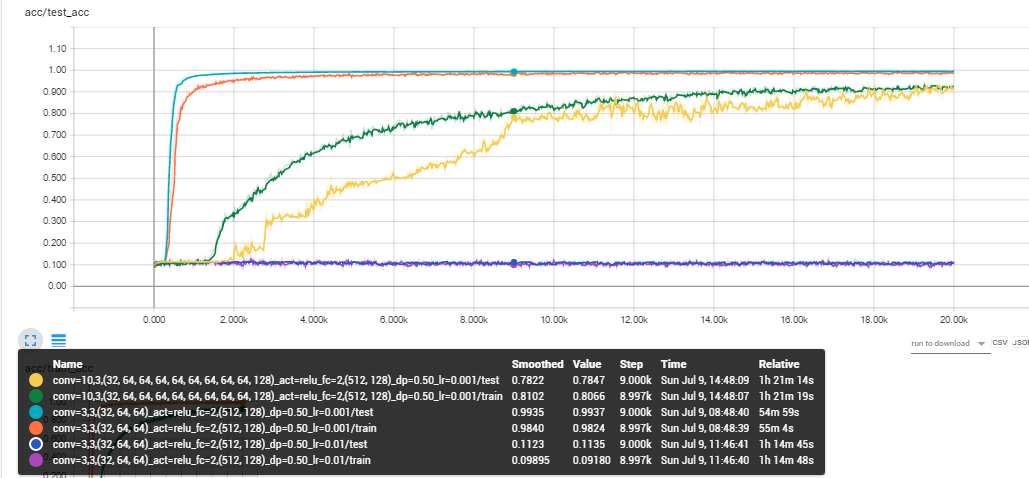
\includegraphics[width=.9\columnwidth]{mnist_lc}	\label{fig:mnist0}} \\
		\subfloat[Parameters of Model with pathological learning rate almost no change]{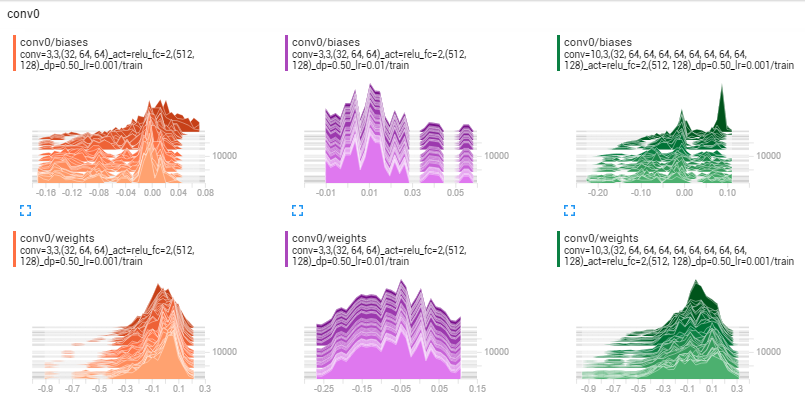
\includegraphics[width=.95\columnwidth]{mnist_conv1}\label{fig:mnist2}} \\ 
		\subfloat[Compared with fig. \ref{fig:mnist2} weights are more smoothed and Gaussian-liked]{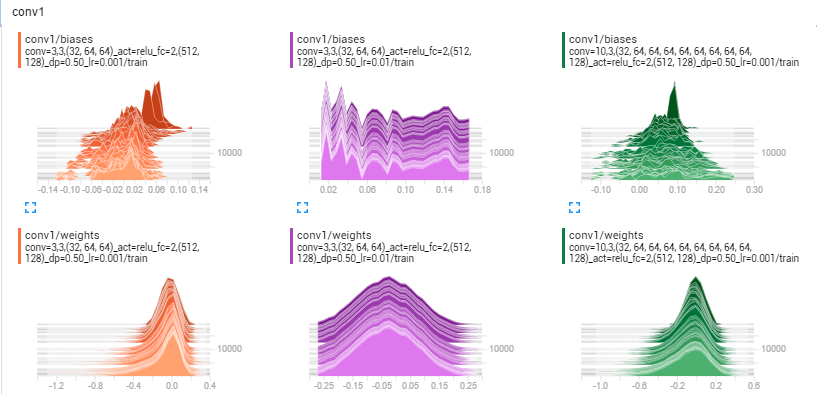
\includegraphics[width=.95\columnwidth]{mnist_conv2}	\label{fig:mnist3}} \\ 
		\caption{Experiments on Mnist} 
		\label{fig:mnist}
\end{figure}

Admittedly, the evolution patterns of parameters and correlations with performance are subtle and need to be captured by some non-linear function. \cite{sinha2017introspection}  use a simple 1-layered Feed-forward Neural Net but leave many questions unanswered:
\begin{itemize}[noitemsep]%[noitemsep,topsep=0pt]
	\item How can architecture and hyper-parameter of forecasting network be  determined(tuned) persuasively? (\cite{baker2017practical} use random search to find best SVM to predict performance) 
	\item How to deal with arbitrary long time series from training history, instead of sampled at $0,4t/10,7t/10,t$? 
	\item How to take relation between the weights into consideration for joint prediction, instead of predict the weights(performance for our task) independently?
\end{itemize}

%Solution: ...

\subsection{Suitability for a Linear Classifier} 
Alain et. al.  \cite{alain2016understanding} re-define information as Suitability for a Linear Classifier/  Separability of Representation/ Computation Complexity rather than Entropy. Though expressed in different means, it can be viewed as prediction error using the features from intermediate layer. 

The \href{ https://youtu.be/x8j4ZHCR2FI }{dynamic}  of probed signals  can also be considered as  hand-crafted feature for performance prediction.  \cite{alain2016understanding} gives some pathological example of Neural Network whose strangeness can be easily identified from dynamics of probed signals.

Meanwhile, it seems that the probed signal    still cannot be explained clearly. For example, if the prediction errors are  as what shown in fig. \ref{fig:probe1}, then we may declare that classification using features from below branch is enough(\textit{i.e.} information only comes from below branch and  above branch is \textit{useless}.). However,   
Alain et. al. argues that features come from above branch is \textit{useful}, because  the prediction error may be noisy and loss can still reduce with concatenated feature.  Admittedly, combined features tend to be useful(or may be redundant), but how can it be conclude from probed signals convincingly? The weakness of probed signal lies in the locality and non-optimality nature, thus hand-crafted feature may not be the best way to observe subtle dynamics.

\begin{figure}[h]
	\centering
	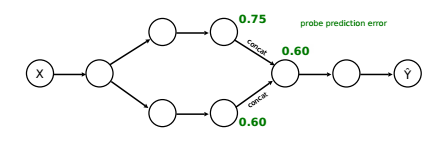
\includegraphics[width=.5\columnwidth]{probe1}
	\caption{Predicion Error of \textbf{Above branch}: 0.75, \textbf{Below branch}: 0.60, \textbf{Concatenated}: 0.60}
	\label{fig:probe1}
\end{figure}

\subsection{Architecture \& Hyper-parameter }
While the general representation of Neural Network is Directed Acyclic Graph/Neural Fabric, Baker et. al. \cite{baker2017practical} extract hand-crafted features $u_\mathbf{x}$ from Neural Net Architecture $\mathbf{x}$, which are simply \textit{total number of weights}, \textit{type and number of layers} and \textit{learning rate}. These features contain very limited information about Neural Net Architecture. Finding optimal numerical representation for  Architecture and Hyper-parameter  is of great necessity. 

%Feature performance experiments with ν-SVR shows that Time-series of validation accuracy is the most informative, however, we should take learning rate into input features and learn a mapping function from   learning rate to performance if we want to automatically tune hyper-parameter like learning rate. 

\subsection{Learning Curve}
Existed work using SVM \cite{klein2016learning}, or BNN \cite{baker2017practical} to predict performance  assume that there is some smooth but noisy function mapping from hyper-parameters(and Statistic,  Hyper-parameter) to the objective. 

SVM outperforms BNN, because BNN learns globally from both  fully observed learning curves(used as training data) and partially observed learning curves(without knowing final performance, used when inference), lacks the ability to make full use of partially observed learning curves  and inferences locally. And it may  suffer from underfitting because of regularization  and potentially wrong prior on weights. 

BNN can inference flexibly without/with partially observed learning curve, and the percentage of observed learning curve need not to be fixed in advance, because BNN also use Architecture and Hyper-parameter to inference and there are some similarity between different setting.  However, SVM assumes fix-length  input features and  need to be retrained when different percentage of observed curves given. 

The weakness of using \textit{only} learning curve lies in: view  Neural Network as a black box, cannot predict precisely. Although experiments with SVM($\nu$-SVR) \cite{baker2017practical} shows that learning curve(validation accuracy) is the most informative on \textit{the dataset they constructed}, statistic from weight and dynamic inside Neural Network should count a lot. The high performance in \cite{baker2017practical} may contribute to the fact that they use training and testing dataset in the same domain, \textit{e.g.} train AlexNet on ImageNet, collect training data, and  only predict  the performance of AlexNet with different hyper-parameter on ImageNet. 

\subsection{Statistical Interactions}
\textit{Main effect} happens when one independent variable affects the dependent variable of interest; \textit{Interactions} happens when multiple independent variables influence the  dependent variable of interest in non-additive fashion. 

Tsang et. al. \cite{tsang2017detecting} propose a method to detect interaction between activations with little modification to Network. 
First, \textit{adjust the network architecture} to directly model main effects as separate
components in the network, as illustrated in fig. \ref{fig:det_stat}. The righthand primary Neural Network is the original network, and interaction can be easily detect from the weights in network.

\begin{figure}[h]
	\centering
	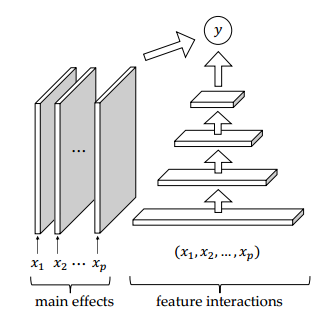
\includegraphics[width=.5\columnwidth]{det_stat} 
	\caption{\textbf{Lefthand}: capture Main Effect; \textbf{Righthand}: Original Network and will be detected interaction relation}
	\label{fig:det_stat}
\end{figure}

Assume $i$ is the common neural unit, $\mathcal{I}$ is the set of interactive neural units, then the importance of interaction is evaluated as   $\omega_i(\mathcal{I})=z_i \omega (\mathcal{I}, \mathbf{W}_{i,:} ) $, 
where $\omega(\mathcal{I} ,\mathbf{W}_{i,:})  =  min_{j \in \mathcal{I}} \{ |\mathbf{W}_{i,j}| \} $ measures the interaction strength at $i$ and
$z^{(l)} = |\mathbf{w}|^T  \left| \mathbf{W}^{(L)} \right|   \left| \mathbf{W}^{(L-1)} \right|  \cdots  \left| \mathbf{W}^{(l+1)} \right|   $ measures the strength after $i$. Apparently, the statistical interactions only depend on weights. 

Applying this method, Tsang et. al. cannot detect interaction between feature map in deep hidden layers, and they guess that neural network mainly uses its early hidden layers to model interactions
and its later layers to model the nonlinearities of these interactions. 

%\section{Learning Features}
 
\section{Necessity of Holistic Hyper-Parameter Tuning}
We defines hyper-parameter as parameters that  cannot be directly learned from the regular training process. They express "higher-level" properties of the model such as its complexity(Architecture of Model) or how fast it should learn(Learning Rate). While search for optimal model often concerned in Meta-modeling, we  focus on \textit{Hyper-parameter of optimization algorithm} \footnote{The hyper-parameter for  optimization algorithm include Learning Rate, Momentum, Learning Rate Decay, Weight Decay/Weight Regularizer, Parameters in Weight Initialization and Initial parameter for Learning Rate and Momentum} where learning rate is the most important concluded by enough tunning experiences.  (Meanwhile, gradient descent optimization algorithms such as RMSprop and Adam compute adaptive learning rates for \textit{each} parameter). 

It is observed \cite{smith2017cyclical} that adaptive learning rate optimizer such as RMSProp and Adam tend to adjust learning rate for short-term benefits. Large learning rate may have short term negative effect and yet achieve a long term benefits. An intuitive understanding is that increasing the learning rate allows more
rapid traversal of saddle point plateaus.  Smith et. al. \cite{smith2017cyclical} use the simplest method but conduct ablation experiments. They use Cyclical Learning Rates where maximum and minimum bound and stepsize is determined from initial epochs of network training, called "LR range test". 

Thus, we may need some holistic method to adjust learning rate for both convergence speed and optimal value where performance prediction  shows its power. 

\section{Potential Future Work}
\begin{itemize}[noitemsep]
	\item Existed work tend to use shallow model as Meta-model to predict performance. We may need to collect diverse training histories and RNN notorious for its sensitivity for Hyper-parameter is worth a try. 
	\item Dynamic Parameters in Neural Network is of attribute size and high dimension(Spatial Dim along layer, Temporal Dim, Width, Height, Channels). Many-to-many combined with many-to-one RNN may be needed. To handle the size, we may need to note that 1). Weights of FC and Conv do not have locality pattern like images. 2). Weights in FC, RNN and Conv are quite different.   3). $S=1,P=0,\frac{W+F+2P}{S}+1=W-F+1$ or Flatten are potential way to handle size, but not the best. 
\end{itemize}

\bibliographystyle{ieee}
\bibliography{library}
	
\end{document}
